%!TEX root = ../docu.tex
\section{Konzept}
\subsection{Grundkonzept}

Im folgenden wird die Konzeptionierung der Anwendung beschrieben ,welche im spteren implementiert wird. heirbei handelt es sich um eine applikation hauptsächlich für das abspielen von Hörbüchern im audioformat MP3. Die applikation soll so einfahc wie möglich gestaltet und zweckgerichtet sein.

die applikation soll dem benutzer ermöglichen hörbücher abzuspielen, welche er vorher auf sein mobiles endgerät abgelegt hat. hierfür muss die applikation einen einstellungsmöglichkeit beinhalten.

über diese einstlelungen muss dem benutzer möglichsein de speicherort frei wählen zu können. über diese einstellungsparameter ist es der anwendung nun möglich alle audiodateien aufzulisten und abspielne zu können.

die auflsitung filtert alle nciht abspielbaren daten und ermöglicht desweitern in unterodernen zu navigieren.

aus dieser auflistung herraus soll es möglich sein audiodateien abspielen zu können.

eine komponente die für das abspielne zuständig ist emfängt die anweisung zum abspielen der audiodatei und spiel dieses datei ab.

\begin{center}
\begin{figure}
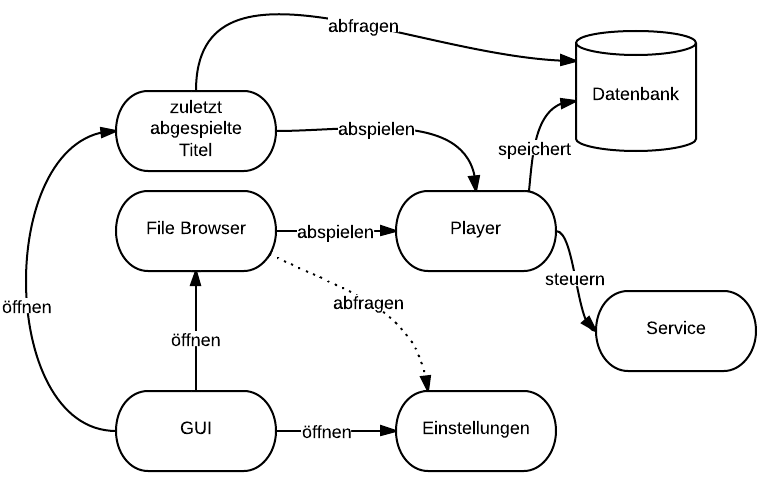
\includegraphics[scale=0.6]{images/konzept}
\caption{Schematische Darstellung der Anwendung}
\label{konzept}
\end{figure}
\end{center}

wird die anwendung geschlossen soll die wiederdabe nciht abbrechen der nutzer soll immernoch in der lage sein die abgespielte audiodatei zu hören.

die anwendung soll in der alge sein abbrüche der wiedergabe zue rknnen und diese punkte zu speicher. der benutzer soll aus diesen informationen eine möglichkeit haben, an diesen punkten die wiedergabe vorzusetzen.

die gesammte progrmamstruktur muss os aufgebaut sein um eine weiteretwicklung und implementierung neuer funrktionen zu ermöglichen.
